After extracting the user's e-mails, we should be able to analyse the body of the e-mails. To do this we will need a syntactic parser in order to separate the different texts in tokens (in other words, to segment text into words, punctuation marks, etc.) and obtain different characteristics from them (such as their part of speech) for the purpose of being able to calculate the metrics explained in Section \ref{ssect:stymet}. To attain that objective, we are going to use the library spaCy\footnote{\url{https://spacy.io/}}.

In this section we are going to explain the reasons why we chose spaCy (see Section \ref{ssect:spacywhy}) and its usefulness in our work (see Section \ref{ssect:spacyut}).

\subsection{spaCy versus others syntactic parsers}\label{ssect:spacywhy}

We have chosen spaCy as our syntactic parser against others for several reasons, supported by published researches (such as the one carried out by \cite{choi2015depends}), that we will explain below.

\begin{figure}[h]
	\centering%
	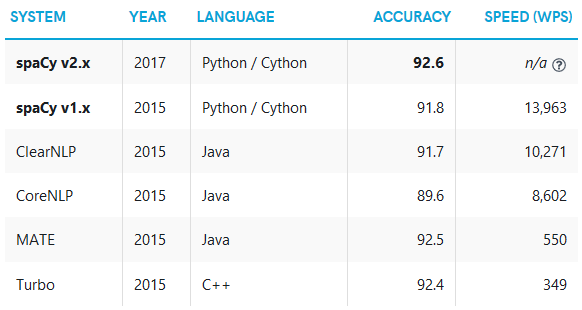
\includegraphics[width = 0.75\textwidth]{Imagenes/Bitmap/Spacy/spacyeval.png}%
	\caption{Benchmarks of different syntactic parsers}%
	Image extracted from \url{https://spacy.io/usage/facts-figures#benchmarks}
	\label{fig:spacyeval}
\end{figure}

An evaluation published by \textit{Yahoo! Labs} and Emory University, as a part of a survey of current parsing technologies \citep{choi2015depends}, observed that ``spaCy is the fastest greedy parser'' and its accuracy is within 1\% of the best available (as we can see in Figure \ref{fig:spacyeval}). The few systems that are more accurate are 20 times slower or more. Speed is an important factor when we want to implement complex systems that are faced with long texts or a large number of documents (as is our case, where we want to analyse all possible e-mails).

\begin{figure}[h]
	\centering%
	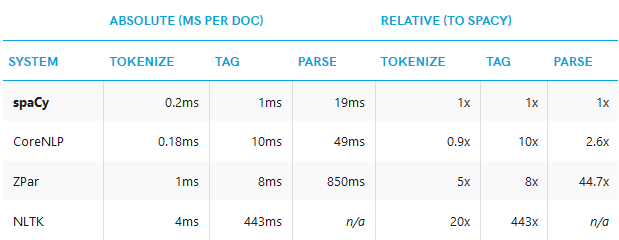
\includegraphics[width = 0.85\textwidth]{Imagenes/Bitmap/Spacy/spacyspeed.png}%
	\caption{Per-document processing time of various NLP libraries}%
	Image extracted from \url{https://spacy.io/usage/facts-figures#benchmarks}
	\label{fig:spacyspeed}
\end{figure}


\cite{choi2015depends} results and subsequent discussions helped spaCy develop a novel psychologically-motivated technique to improve spaCy's accuracy, which they published in joint work with Macquarie University \citep{honnibal2015improved}. For this reason we have chosen spaCy v2.2.1 which takes advantage of this technique.

Furthermore, not only in general but in each particular task (tokenisation, tagging and parsing), spaCy is the fastest if we compare it with other natural language processing libraries. This is shown in Figure \ref{fig:spacyspeed}, where we can observe both absolute timings (in ms) and relative performance (normalized to spaCy). The systems which have lower values are faster in their tasks.

Finally, spaCy has three pretrained model pipelines for Spanish with a very high accuracy (see Figure \ref{fig:spacymodel}). These will help us to tokenise, tag and parse our messages in order to calculate the different style markers defined.

\begin{figure}[h]
	\centering%
	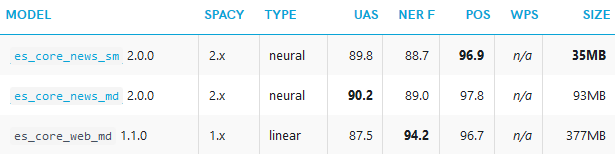
\includegraphics[width = 0.85\textwidth]{Imagenes/Bitmap/Spacy/spacymodel.png}%
	\caption{Benchmark accuracies for the Spanish pretrained model pipelines}%
	Image extracted from \url{https://spacy.io/usage/facts-figures#benchmarks}
	\label{fig:spacymodel}
\end{figure}

\subsection{spaCy's utilities}\label{ssect:spacyut}
We can define spaCy as a Python natural language processing library specifically designed to be a useful library for implementing production-ready systems. For this reason, it has a lot of different utilities. However we are only going to need the ones carried out by the \textit{Tokenizer} and the \textit{Sentencizer}.

The spaCy's \textit{Tokenizer} class is in charge dividing the given message into the different words that constitute it and obtaining several features about them. We are interested in the attributes that we can observe in Table \ref{tab:attspacy}. In addition to its part of speech, it gives us more information (that we are not interested in it) depending on its lexical category, such as its gender, number, verb tense or, even, the type of adverb.

\begin{table}[h]
	\begin{tabular}{|l|l|p{0.675\linewidth}|}
		\hline
		\textbf{Attribute} & \textbf{Type} & \textbf{Explanation}                                                                     \\ \hline
		is\_punct          & bool          & It indicates whether the token is a punctuation mark.                                    \\ \hline
		is\_right\_punct   & bool          & It indicates whether the token is a right punctuation mark (such as a right quote mark). \\ \hline
		is\_left\_punct    & bool          & It indicates whether the token is a left punctuation mark.                               \\ \hline
		is\_bracket        & bool          & It indicates whether the token is a bracket.                                             \\ \hline
		like\_url          & bool          & It indicates whether the token is an url.                                                \\ \hline
		like\_email        & bool          & It indicates whether the token is an e-mail address.                                     \\ \hline
		lema\_             & string        & Base form of the token, with no inflectional suffixes.                                   \\ \hline
		is\_stop           & bool          & It indicates whether the token is a stop word.                                           \\ \hline
		pos\_              & string        & Part of speech of the token.                                                             \\ \hline
		is\_oov			   & bool		   & It indicates whether the token is recognised by our spaCy's model and it has information about it\\ \hline
		text & string & Verbatim text content. \\ \hline
		idx & integer & The character offset of the token within the parent document. \\ \hline
	\end{tabular}
	\caption{\textit{Tokenizer}'s interesting attributes}\label{tab:attspacy}
\end{table}
 
 The spaCy's \textit{Sentencizer} class is in charge of establishing the boundaries between each sentence of the text. In this way, we are able to calculate metrics such as the average length of the sentences of the document.